% pdf/a 
\begin{filecontents*}[overwrite]{\jobname.xmpdata}
	\Title{Koncentrált paraméterű RF szűrő optimalizációja aktív tanulással}
	\Author{Pintér Bálint, Szilágyi Gábor}
	\Language{hu-HU}
	\Subject{Bayes-optimalizáció}
	\Keywords{Bayes-optimalizáció, aktív tanulás}
	\Publisher{Pintér Bálint, Szilágyi Gábor}
\end{filecontents*}

\documentclass[a4paper,12pt,titlepage]{article}
%\documentclass[a4paper,12pt,titlepage,draft]{article}
%\usepackage{ucs}
\usepackage[T1]{fontenc}
\usepackage[utf8]{inputenc}
\usepackage[magyar]{babel}
\usepackage{amsfonts}
\usepackage{amsmath,bm}
%\usepackage{mathtools} % for \ceil*{}
\usepackage{amssymb}
\usepackage{graphicx}
\usepackage{csquotes}
%\usepackage[hang]{caption}
\usepackage{subcaption}
\usepackage{blkarray,booktabs,bigstrut} % a címkézett mátrixhoz
%\usepackage{enumerate}
%\usepackage{psfrag}
\usepackage[left=25mm,right=25mm,top=25mm,bottom=25mm]{geometry}
%\usepackage[hyphenbreaks]{breakurl}
%\usepackage[hyphens]{url}
%\usepackage{multirow}
%\usepackage{booktabs}
%\usepackage[square,numbers]{natbib}
\usepackage{circuitikz}
\usepackage{hyperref}
\usepackage{listings}
%\usepackage{cite}
%\usepackage{csquotes}
%\usepackage{inconsolata}
\usepackage{siunitx}
\usepackage{xcolor}
\usepackage[a-3u]{pdfx}
\hypersetup{
	colorlinks,
%	 linkcolor={red!50!black},
	linkcolor={black},
%	 citecolor={blue!50!black},
	citecolor={black},
%	 urlcolor={blue!80!black}
	urlcolor={blue!80!black}
}

\definecolor{mygray}{RGB}{240, 240, 240}
\definecolor{mygreen}{RGB}{0, 140, 40}

% ez nekem valamiért akad, bocsi, hogy kiszedtem
\sisetup{range-phrase=--,
        range-units=single,
        output-decimal-marker={,},
        tight-spacing=true,
%        print-unity-mantissa=false,
        }

\lstset{ % General setup for the package
	language=Python,
	basicstyle=\scriptsize\ttfamily,
	numbers=left,
	numberstyle=\tiny,
	tabsize=2,
	backgroundcolor=\color{mygray},
	columns=fixed,
	showstringspaces=false,
	showtabs=false,
	keepspaces,
	frame=trbl,
	breaklines=true,
	%breakwhitespace=true,
	morekeywords={sort2,sort8},
	stringstyle=\color{red},
	commentstyle=\color{mygreen},
	keywordstyle=\color{blue}
}

\sloppy % Margón túllógó sorok tiltása.
\widowpenalty=10000 \clubpenalty=10000 %A fattyú- és árvasorok elkerülése
\def\hyph{-\penalty0\hskip0pt\relax} % Kötőjeles szavak elválasztásának engedélyezése

\newcommand\vect[1]{\underline{#1}}
\newcommand\mat[1]{\underline{\underline{#1}}}

\title{
    \huge{Neurális hálózatok házi feladat beszámoló} \\
	\vspace*{2cm}
	\large{Pintér Bálint (I6QS0K), Szilágyi Gábor (NOMK01)}\\
	\vspace*{2cm}
	\Large{Koncentrált paraméterű RF szűrő optimalizációja \\ aktív tanulással}
}

\begin{document}
\maketitle
\tableofcontents
\section{Bevezetés}
	\subsection{Aktív tanulás}
		A legtöbb neurális hálózatokat használó megoldás olyan problémára irányul, ahol sok rendelkezésre álló adat alapján kell a hálót betanítani egy feladat elvégzésére. Az a legtöbb esetben teljesül, hogy még több tanító adat felhasználásával jobb hálót lehetne tanítani, de ennek az extrém esetére tud megoldást nyújtani az aktív tanulás. A nem adathiányos problémáknál a rendelkezésre álló, címkézett adatpontok nagy részét felhasználva szokás tanítani a hálót, majd a fennmaradó adatpontokon ellenőrizni a háló teljesítőképességét olyan esetekre, amikkel nem találkozott a tanulás során. Az aktív tanulás folyamata ettől merőben eltér.

		Aktív tanulás kiindulási helyzete, hogy nagyon sok címkézetlen adat áll rendelkezésre, de az egyes adatpontok címkézése rendkívül költséges. A címkézés költsége miatt végeredményben az a cél, hogy azt minél kevesebbszer kelljen elvégezni a tanulás során. A tanulási folyamat közben az eddig megkapott kevés címkézett adatpont alapján a háló jelöl ki következőnek címkézésre azt, amelyik várhatóan a leghasznosabb lesz számára. A hasznosság becslésére több megközelítés is létezik, erre a későbbiekben visszatérünk.

		Az aktív tanulás egyik alesete a Bayes-optimalizáció. Itt nem egy osztályozót tanítunk minél kevesebb címkézett adat alapján, hanem egy ,,fekete doboz'' függvény maximumát keressük a függvény minél kevesebb kiértékelése mellett. Ez a különbség már befolyásolni fogja a következőnek megcímkézendő adat választását, ami ebben az esetben a következő paraméterértékek megválasztását jelenti, ahol kiértékeljük a függvényt.
	\subsection{Az optimalizálandó probléma}
		Az optimalizálandó probléma egy koncentrált paraméterű rádiófrekvenciás (RF) szűrő elemeinek megadása, azaz méretezése. Egy koncentrált paraméterű elemekből felépülő szűrő alapesetben ellenállásból, tekercsekből és kondenzátorokból áll, de léteznek aktív elemet, azaz erősítőt is tartalmazó szűrők -- de ez már kívül esik a vizsgálatunkon, csak passzív eszközökkel foglalkozunk. Feltesszük továbbá, hogy a vizsgálatunk során csillapítással nem foglalkozunk, így ellenállást sem használunk a szűrőnkhöz.
		
		Szűrőtervezéskor mindig egy előre megadott specifikációból indulunk ki, ebben elő van írva azon frekvenciatartományok csoportja, ahol a szűrni kell, illetve ahol csillapítás nélkül kell az RF teljesítményt átereszteni. Ennek megfelelően beszélhetünk záró és áteresztő sávokról, ahol a szűrő impedanciakarakterisztikájának rendre nagynak, illetve kicsinek kell lennie, ehhez a tekercsek és kondenzátorok soros és párhuzamos rezonanciáit használjuk ki. (S paraméter majd később).
		
		A valóságban mind a tekercsek, mind a kondenzátorok 3D-s objektumok, induktivitásuk és kapacitásuk anyagparamétertől és geometriai méretektől függenek. Anyagparamétertől függés alatt a kondenzátorok dielektrikumában a relatív permittivitását, illetve a tekercsek belsejében a közeg relatív permeabilitását kell érteni -- bár utóbbi nem jellemző RF szűrők esetében. Az anyagparaméter tehát egy fix érték, amit nem egyszerű változtatni, méretezés céljából ez nem járható út. Megoldást a geometriai méretek optimális megválasztása jelent, ami utat nyit az alapesetektől, az analitikus formulákkal egyszerűen kiszámolható geometriáktól való eltéréshez. Bár ezekben az alapesetekben, a síkkondenzátorban és az egyenes tekercsben, a szolenoidban is megjelennek geometriai jellemzők, a
\begin{align*}
	C &= \varepsilon_{0}\varepsilon_{r}\frac{A}{d}\\
	L &= \mu_{0}\mu_{r}\frac{N^{2}A}{l}
\end{align*}
formulák egyrészt csak közelítések, azaz nem írják le pontosan az $L$ és a $C$ értékeket, másrészt sokszor nem kivitelezhető az általuk leírt komponens.
		
		A feladat innentől az, hogy olyan geometriai méreteket találjunk, amivel a komponensek pont az általunk kívánt $L$ és $C$ értékeket mutassák, ezzel a specifikációnak eleget tudjunk tenni. Esetünkben a nem analitikusan kiszámolható értékekhez numerikus megoldást kell keresni, amire egy jó megoldás, ha 3D véges elemes szimulációt készítünk. Egy-egy szimuláció futási ideje a megkövetelt precizitás és a rendelkezésünkre álló erőforrás függvényében változhat, de mindenképp több mint csupán egyetlen egyenlet kiértékelése. Éppen ezért szükséges az optimalizálást úgy végezni, hogy szempont legyen a minél kevesebbszer történű kiértékelés. 
		
		A fent leírtak az RF szűrőtervezés témakörében egy releváns problémát takarnak, munkánkban azonban nem 3D véges elemes szimulációkat használunk, nem geometriai paraméterek optimalizálását végezzük el. Tesszük mindezt egyrészt azért, mert a szimulációs szoftverek programozott vezérlése meglehetősen nehéz, másrészt a neurális hálók szempontjából teljesen lényegtelen, hogy a kiértékelt függvényben mi történik. Azonban maga az optimalizálás amit csinálunk alkalmas egy ilyen feladatra, és érdemben tudja a tervezőt segíteni munkája során. Visszatérni tehát a koncentrált paraméterű, $L$ és $C$ elemeket tartalmazó hálózatra az optimalizáció szempontjából nem jelent kevesebb munkát, ebben az értelemben nem jár a feladat egyszerűsítésével.
		
		A feladathoz már csak egy lépés hiányzik, amivel a problémát át tudjuk alakítani egy szélsőérték keresésre. Ennek az alapgondolata az, hogy az elvárt és a kapott kimenet különbségét vesszük figyelembe egy büntetőfüggvény segítségével. Magát az optimalizálást ezen keresztül tudjuk megtenni, ennek a függvénynek a kifejtésére a \ref{sec:celfuggveny}. részben kerül sor.
		
	\subsection{A felhasznált könyvtár}
	
		Bayes-optimalizáció megvalósításához már léteznek elkészített könyvtárak, így azt külön nem készítettük el, hanem felhasználtuk. Az általunk használt ingyenesen elérhető és letölthető \textit{Bayesian Optimization} könyvtár más, neurális hálózatokra készített, ugyancsak szabadon hozzáférhető könyvtárakon alapszik \cite{scipy}, itt most ennek a bemutatását adjuk \cite{lancpar_spar}.
		
		A \textit{Bayesian Optimization} használata rendkívül egyszerű, összesen két dolgot kell megtennünk. Elsőként példányosítjuk a \textit{BayesianOptimization} osztályt, ami bemeneti paraméterként megkapja a maximalizálandó költségfüggvényt, illetve a határait annak a tartománynak, ahol a maximumot keresnie kell. Fontos kiemelni, hogy esetünkben a kapott és az elvárt kimenetek közötti minimalizálás a feladat, így a költségfüggvényben át kell térni maximumhely keresésre. 
		
		A szélsőértékhely keresést ezután a \textit{maximize( )} tagfüggvény hajtja végre. Ez a folyamat kezdetben random helyeken kiértékel pontokból indul el, majd iteratívan halad a modelltérben az optimum felé. Ennek megfelelően a \textit{maximize( )} bemeneti paraméterei az inicializáló, véletlenszerű helyek száma és az iteráció száma. Ebben elsőként példányosul egy \textit{UtilityFunction} nevű osztály, utána elindul az iteráció. 
		Minden kör az előző lefutás utáni paraméterfrissítéssel, az \textit{update\_param( )}-mal kezdődik, ami a \textit{UtilityFunction} egy tagfüggvénye. A függvénynek több felderítési típusa lehet, ezek a UCB (Upper Confidence Bounds method), az EI (Expected Improvement method) és a POI (Probability Of Improvement), alapesetben az UCB-t használjuk. Az \textit{update\_param( )}-nak három hiperparamétere van: $\chi$, $\kappa$ és $\kappa_{decay}$, az utóbbi a $\kappa$ csökkentését végzi minden iterációban, de csak egy másik paraméter, $\kappa_{delay}$ iterációtól kezdve.
		Frissítve a \textit{UtilityFunction}-t, egy javaslattevő tagfüggvénynek, a \textit{suggest( )}-nek adjuk át inputként, ami javasol egy új pontot, az \textit{x\_probe}-ot a következő kiértékelésre. Ebben a \textit{suggest( )}-ben egy \textit{argmax} vizsgálat történik egy akvizíciós függvényre, az \textit{acq\_max}-ra. Ez a vizsgálat két lépésből áll, elsőként egyenletes eloszlással felvesztünk mintavételi pontokat a \textit{UtilityFunction}-ból a paramétertartomány határain belül, alapbeállításként $10^{5}$ darabot. Második lépésként \textit{L-BFGS-B} optimalizációs metódus futtatunk le minden mintavételezett pontra. Egy ciklusban kiválasztjuk a legnagyobbat, ezzel térünk vissza, ez lesz \textit{x\_probe}, a javasolt új kiértékelési hely.
		A \textit{maximize( )} iterációs ciklusának harmadik lépése maga a kiértékelés, erre a \textit{probe( )} tagfüggvény szolgál, ami az általunk megadott költségfüggvényt futtatja le a kiszámolt új \textit{x\_probe} helyen. Ezt a három iterációs lépést folytatja a kód a meghatározott iterációszámig.
	
		Az \textit{L-BFGS-B} optimalizáló solver nem ebben a könyvtárban van megírva, hanem a \textit{scipy.optimizer} tartalmazza \cite{scipy}. Ez egy minimalizálási feladatokra készített másodrendű optimalizációs algoritmus, az \textit{L-BFGS} kiterjesztése korlátok kezelésére. Feloldva a rövidítést a Limited-memory Broyden-Fletcher-Goldfarb-Shanno algoritmus egy kvázi-Newton módszer, másodrendű deriváltak közelítésére hasznos, ahol az közvetlenül nehéz kiszámolni. Konkretizálva ez azt jelenti, hogy nem számolja ki a Hesse-mátrixot, csak annak inverzét közelíti. A módszer nevében az L előtag a limitált memóriára utal, azaz mindig csak az elmúlt $m$ lépés koordináta- és gradiensvektorát tárolja el. Ez a memóriagazdálkodás fontos, különösen az \textit{acq\_max} függvényben, ahol mind a $10^{5}$ mintavételi pontra elvégezzük az \textit{L-BFGS-B}-t.
	
\section{A célfüggvény felírása}
\label{sec:celfuggveny}
    A célfüggvényünket olyan formában definiáltuk, hogy az adott specifikációnak jobban megfelelő szűrőparaméterekhez nagyobb számot rendeljen. A specifikációban frekvenciasávok és a hozzájuk elvárt minimális vagy maximális átvitel van megadva. Az átvitel itt a teljes kétportú (vagyis négypólusú) rendszer szórási mátrixának (S-mátrixának) egyik elemét, név szerint az $S_{21}$-et jelenti. Mivel ez a reaktív elemek jelenléte miatt egy komplex szám, ennek az abszolút értékét vizsgáljuk, a specifikációbeli korlátok is az abszolút értékre vonatkoznak. Az $S_{21}$ paraméter egy frekvenciafüggő mennyiség, ami azt az információt hordozza, hogy ha az 1-es porton (kapun) beküldünk a szűrőbe egy adott amplitúdójú és frekvenciájú szinuszos feszültséghullámot, akkor az a rendszer 2-es portján milyen amplitúdójú és fázisú kimenő feszültséghullámot eredményez. Az $S_{21}$ komplex fázisa a két feszültséghullám relatív fázisát fejezi ki, ez számunkra nem érdekes, ezért vesszük az abszolút értéket. Ha $|S_{21}|(f) = 1$, akkor a szűrő az adott $f$ frekvencián nem csillapít, de nem is erősít, tehát tökéletesen átereszti a rajta keresztülküldött jelet, legfeljebb más fázisban. Ez lenne a szűrő ideális viselkedése áteresztő sávban. Ha pedig $|S_{21}|(f) = 0$, akkor a beküldött jelből semmit nem enged át, azt általános esetben vagy elnyeli, vagy visszaveri, de mivel mi veszteségmentes, LC szűrőkkel foglalkoztunk, itt az elnyelés nem jöhet szóba. Ez utóbbi pedig az ideális viselkedés záró sávban. Természetesen véges frekvencián és véges elemértékekkel egyik szélső eset sem megvalósítható, még az ideális LC komponensekkel sem, amelyekkel mi számolunk. A szűrő tehát mindig valamilyen 0 és 1 közötti $|S_{21}|$-et fog mutatni bármilyen frekvencián és bármilyen behelyettesített elemértékek mellett.

    A célfüggvényünket, vagyis $c(\vect{x})$-t, ahol $\vect{x}$ a behelyettesített elemértékek vektora, egy összeggel definiáljuk. Az összegben diszkrét frekvenciákon felvett hibaértékeket, $h(f,\vect{x})$-ket adunk össze.
    \begin{equation}
        c(\vect{x}) = \sum_{i=1}^{N_f} h(f_i,\vect{x})
    \end{equation}
    A vizsgált diszkrét $f_i$ frekvenciákat logaritmikusan vettük fel a legkisebb és a legnagyobb specifikált frekvencia között, a kiértékelt frekvenciák száma, $N_f$ megadható a specifikáció definiálásakor a programunkban. Ha egy adott frekvencián a kiszámolt $S(f)=|S_{21}|(f)$ kisebb, mint a megadott maximum, $S_{max}(f)$ vagy hasonlóan, ha nagyobb, mint a megadott minimum, $S_{min}(f)$, akkor a célfüggvény értékét nem változtatjuk az $f_i$ frekvencián mutatott viselkedés alapján, itt nem büntetünk. Ez egyben azt is jelenti, hogy az adott diszkrét frekvencián megfelel a specifikációnak a szűrő. Ellenkező esetben minél jobban belóg az $S(f)$ a tiltott zónába, annál nagyobb abszolút értékű negatív szám lesz $h(f,\vect{x})$ értéke. A fent vázolt összegzős módszerrel egy olyan mennyiséget kapunk, ami az $S(f)$ átviteli függvény tiltott zónákba való belógásának integrálját közelíti. Hogy ez a belógás, vagyis a $h(f,\vect{x})$ pontosabban mit takar, később fejtjük ki \aref{sec:celfuggveny_javitas}. fejezetben.
    \subsection{A hálózat kapcsolási rajza}
        A hálózatnak gyakorlatilag a kapcsolási rajza adott L és C elemértékekkel, innen kell valahogyan eljutni az $|S_{21}|$ paraméterig. Olyan struktúrájú szűrőt választottunk, amivel szűrőkarakterisztikák széles köre megvalósítható. Alapvetően egy periodikus szerkezetű kapcsolásról van szó, de az egyes blokkokban, amik egymás után vannak kapcsolva, külön meg lehet adni az elemértékeket, eleve azt is, hogy az adott pozícióban van-e kondenzátor vagy induktivitás. A programkódunk végleges verziójában legfeljebb 3 db ilyen blokk használható, de a kód minimális módosításával bővíthető még több blokkal szükség szerint. Egy ilyen blokk kapcsolási rajza \aref{fig:egyseg_kapcsolas}. ábrán látható.
        \begin{figure}
            \centering
            \begin{circuitikz}[] %[longL/.style = {cute inductor, inductors/scale=0.75, inductors/width=1.6, inductors/coils=9}]
                \draw (-0.5,0)
                to[short, o-*] (2,0)
                to[short, -*] (2,0.5)
                to[short, -] (1,0.5);
                \draw (1,2.5)
                to[C, l=$C_{i,p}$] (1,0.5);
                \draw (2,2.5)
                to[short, -] (3,2.5)
                to[L, l=$L_{i,p}$] (3,0.5)
                to[short, -] (2,0.5);
                \draw (-0.5,3)
                to[short, o-*] (2,3)
                to[short, -*] (2,2.5)
                to[short, -] (1,2.5);
                \draw (2,0)
                to[short, -o] (8,0);
                \draw (2,3)
                to[short, -*] (5,3)
                to[short, -] (5,2)
                to[L, a=$L_{i,s}$] (7,2)
                to[short, -] (7,3);
                \draw (5,3)
                to[short, -] (5,4)
                to[C, a=$C_{i,s}$] (7,4)
                to[short, -*] (7,3)
                to[short, -o] (8,3);
                \draw[thick,red] (0,-0.5) rectangle (7.5,5);
                \draw (-1,1.5) node{1. port};
                \draw (8.5,1.5) node{2. port};
            \end{circuitikz}
            \caption{Az optimalizálandó szűrő $i$-edik egysége}
            \label{fig:egyseg_kapcsolas}
        \end{figure}
        Ahogy az ábrán is látszik, az egységhálózat egy kétkapu, amiben egy párhuzamos és egy soros LC rezgőkör van. Ez csak abban az esetben néz ki pontosan így, ha mind a négy paraméterértéket beállítjuk. Ha egyes komponenseket nem használunk, akkor azokat szakadással, vagy rövidzárral helyettesíti a program, ahogy annak a teljes hálózat szempontjából értelme van. Erre láthatunk néhány példát \aref{fig:egyseg_parh_LC}. \ref{fig:egyseg_sor_LC}. és \ref{fig:egyseg_alulatereszto}. ábrán.
        \begin{figure}
            \centering
            \begin{circuitikz}[] %[longL/.style = {cute inductor, inductors/scale=0.75, inductors/width=1.6, inductors/coils=9}]
                \draw (-0.5,0)
                to[short, o-*] (2,0)
                to[short, -*] (2,0.5)
                to[short, -] (1,0.5);
                \draw (1,2.5)
                to[C, l=$C_{i,p}$] (1,0.5);
                \draw (2,2.5)
                to[short, -] (3,2.5)
                to[L, l=$L_{i,p}$] (3,0.5)
                to[short, -] (2,0.5);
                \draw (-0.5,3)
                to[short, o-*] (2,3)
                to[short, -*] (2,2.5)
                to[short, -] (1,2.5);
                \draw (2,0)
                to[short, -o] (8,0);
                \draw (2,3)
                to[short, -*] (5,3)
                to[short, -] (5,2)
                to[short, -] (7,2)
                to[short, -] (7,3);
                \draw (5,3)
                to[short, -] (5,4)
                to[openbarrier] (7,4)
                to[short, -*] (7,3)
                to[short, -o] (8,3);
                \draw[thick,red] (0,-0.5) rectangle (7.5,5);
            \end{circuitikz}
            \caption{Az egységhálózat párhuzamosan kötött párhuzamos LC rezgőkörnek használva. Itt érdekesség, hogy a soros ágban egyik alkatrészt sem használjuk, mégis összesen egy rövidzárral vannak helyettesítve, mivel ennek a helyettesítésnek van értelme.}
            \label{fig:egyseg_parh_LC}
        \end{figure}
        \begin{figure}
            \centering
            \begin{circuitikz}[] %[longL/.style = {cute inductor, inductors/scale=0.75, inductors/width=1.6, inductors/coils=9}]
                \draw (-0.5,0)
                to[short, o-*] (2,0)
                to[short, -*] (2,0.5)
                to[short, -] (1,0.5);
                \draw (1,2.5)
                to[openbarrier] (1,0.5);
                \draw (2,2.5)
                to[short, -] (3,2.5)
                to[openbarrier] (3,0.5)
                to[short, -] (2,0.5);
                \draw (-0.5,3)
                to[short, o-*] (2,3)
                to[short, -*] (2,2.5)
                to[short, -] (1,2.5);
                \draw (2,0)
                to[short, -o] (8,0);
                \draw (2,3)
                to[short, -*] (5,3)
                to[short, -] (5,2)
                to[L, a=$L_{i,s}$] (7,2)
                to[short, -] (7,3);
                \draw (5,3)
                to[short, -] (5,4)
                to[C, a=$C_{i,s}$] (7,4)
                to[short, -*] (7,3)
                to[short, -o] (8,3);
                \draw[thick,red] (0,-0.5) rectangle (7.5,5);
            \end{circuitikz}
            \caption{Az egységhálózat sorosan kötött párhuzamos LC rezgőkörnek használva.}
            \label{fig:egyseg_sor_LC}
        \end{figure}
        \begin{figure}
            \centering
            \begin{circuitikz}[] %[longL/.style = {cute inductor, inductors/scale=0.75, inductors/width=1.6, inductors/coils=9}]
                \draw (-0.5,0)
                to[short, o-*] (2,0)
                to[short, -*] (2,0.5)
                to[short, -] (1,0.5);
                \draw (1,2.5)
                to[C, l=$C_{i,p}$] (1,0.5);
                \draw (2,2.5)
                to[short, -] (3,2.5)
                to[openbarrier] (3,0.5)
                to[short, -] (2,0.5);
                \draw (-0.5,3)
                to[short, o-*] (2,3)
                to[short, -*] (2,2.5)
                to[short, -] (1,2.5);
                \draw (2,0)
                to[short, -o] (8,0);
                \draw (2,3)
                to[short, -*] (5,3)
                to[short, -] (5,2)
                to[L, a=$L_{i,s}$] (7,2)
                to[short, -] (7,3);
                \draw (5,3)
                to[short, -] (5,4)
                to[openbarrier] (7,4)
                to[short, -*] (7,3)
                to[short, -o] (8,3);
                \draw[thick,red] (0,-0.5) rectangle (7.5,5);
            \end{circuitikz}
            \caption{Az egységhálózat elsőrendű LC aluláteresztő szűrőnek használva.}
            \label{fig:egyseg_alulatereszto}
        \end{figure}
    \subsection{Impedanciák és admittanciák}
        A célfüggvény számításának logikusan következő lépése, hogy az elemértékekből egy-egy diszkrét frekvencián helyettesítő impedanciát számolunk. A kódban egyébként az egyes párhuzamos rezgőkörökre direkte határozzuk meg annak az eredő impedanciát (vagy admittanciát) az \textit{Impedance( )} és \textit{Admittance( )} függvények segítségével. Ezek után a helyettesítőkép \aref{fig:impedancia}. ábrán látható módon alakul.
        \begin{figure}
            \begin{center}
                \begin{circuitikz}[] %[longL/.style = {cute inductor, inductors/scale=0.75, inductors/width=1.6, inductors/coils=9}]
                    \draw (-0.5,0)
                    to[short, o-*] (2,0)
                    to[short, -] (2,0.5);
                    \draw (2,2.5)
                    to[xgeneric, l=$Y_{i,p}(f)$] (2,0.5);
                    \draw (-0.5,3)
                    to[short, o-*] (2,3)
                    to[short, -] (2,2.5);
                    \draw (2,0)
                    to[short, -o] (8,0);
                    \draw (2,3)
                    to[short, -] (5,3)
                    to[xgeneric, a=$Z_{i,s}(f)$] (7,3)
                    to[short, -o] (8,3);
                    \draw[thick,red] (0,-0.5) rectangle (7.5,3.5);
                \end{circuitikz}
            \end{center}
            \caption{Helyettesítő impedancia és admittancia}
            \label{fig:impedancia}
        \end{figure}
        Itt a paraméterértékek az alábbi képletek alapján adódnak. Természetesen külön le vannak kezelve azok az esetek, amikor valamelyik impedancia vagy admittancia 0-ra vagy $\infty$-re adódik és nem lehet direkt behelyettesíteni a képletekbe.
        \begin{align}
            Z_{i,p,L} & = i2\pi f\cdot L_{i,p} \\[3ex]
            Z_{i,p,C} & = \dfrac{1}{i2\pi f\cdot C_{i,p}} \\[3ex]
            Z_{i,s,L} & = i2\pi f\cdot L_{i,s} \\[3ex]
            Z_{i,s,C} & = \dfrac{1}{i2\pi f\cdot C_{i,s}} \\[3ex]
            Z_{i,s} & = \dfrac{Z_{i,s,C}\cdot Z_{i,s,L}}{Z_{i,s,C}+Z_{i,s,L}} \\[3ex]
            Y_{i,p} &= \dfrac{Z_{i,p,C}+Z_{i,p,L}}{Z_{i,p,C}\cdot Z_{i,p,L}}
        \end{align}
	\subsection{Láncparaméterek}
        \label{subsec:lancparameterek}
        A következő lépés egy köztes számítás, ami az egyes egységblokkok kaszkádkapcsolásának számítását könnyíti meg. Ehhez a láncparamétereket hívjuk segítségül, amelyek az angol szakirodalomban ABCD-paraméterekként szerepelnek. A láncparaméterek mátrixa, vagyis $\mat{A} \in \mathbb{C}^{2\times2}$ lényegében a leírt rendszer két portján felvett feszültségek és áramok között teremt kapcsolatot, az impedanciaparaméterekhez (Z-paraméterek) nagyon hasonló módon. Egy adott frekvencián ezzel a $2\times2$-es mátrixszal teljesen leírható a hálózat. A feszültségek és áramok referenciairányai úgy vannak megválasztva a láncparaméterek felírásakor, hogy a kaszkádba kapcsolt kétportú hálózatok eredő láncparamétereit az összekapcsolt alegységek $\mat{A}$ mátrixainak szorzataként kaphatjuk meg, ahogy az \aref{fig:kaszkad}. ábrán látható.
        \begin{align}
            \mat{A} = \prod_{i}^{} \mat{A_{i}} = \begin{bmatrix}a_{11}~a_{12} \\ a_{21}~a_{22}\end{bmatrix} = \begin{bmatrix}A~B \\ C~D\end{bmatrix}
        \end{align}
        \begin{figure}
            \centering
            \begin{circuitikz}[] %[longL/.style = {cute inductor, inductors/scale=0.75, inductors/width=1.6, inductors/coils=9}]
                \foreach \x in {1,...,5}
                {
                    \draw (\x+\x-0.5,0)
                    to[short, o-] (\x+\x+0,0);
                    \draw (\x+\x-0.5,1)
                    to[short, o-] (\x+\x+0,1);
                    \draw[thick,red] (\x+\x+0,-0.2) rectangle (\x+\x+1,1.2);
                    \draw (\x+\x+1,0)
                    to[short, -o] (\x+\x+1.5,0);
                    \draw (\x+\x+1,1)
                    to[short, -o] (\x+\x+1.5,1);
                    \draw (\x+\x+0.5,0.5) node {$\mat{A_{\x}}$};
                }
                \draw[thick,green] (1.75,-0.5) rectangle (11.25,1.5);
            \end{circuitikz}
            \caption{A hálózat egységeinek kaszkád kapcsolása.}
            \label{fig:kaszkad}
        \end{figure}
	\subsection{Szórási paraméterek}
        Végül elérkeztünk a szórási paraméterek számításához. \Aref{subsec:lancparameterek}. pontban tárgyalt láncparaméterek használatát az is indokolja, hogy létezik egyszerű képlet az $\mat{A}$ mátrixból $\mat{S}$ mátrixba való áttérésre. Az $\mat{S}$ mátrix minden elemére külön analitikus képlet van \cite{lancpar_spar}, de mivel nekünk csak az $S_{21}$-re van szükségünk, így csak az erre a konkrét paraméterre vonatkozót kellett használnunk. Az S-paraméterek használatához minden portra definiálni kell egy normalizáló impedanciát, $Z_0$-t. Ezt mi a konvencionálisnak számító $\SI{50}{\Omega}$-ra választottuk. 
    \begin{equation}
        S_{21} = \dfrac{2}{A+B/Z_0+CZ_0+D}
    \end{equation}
\section{A célfüggvény javítása}
    \label{sec:celfuggveny_javitas}
    A $c(\vect{x})$ célfüggvény a félév során átesett néhány változtatáson. Ezt az indokolta, hogy a naívan, első próbálkozásként felírt célfüggvény több szempontból sem viselkedett jól az optimalizálás szempontjából. Ebben a fejezetben ezeket a fejlesztési lépéseket írjuk le.
	\subsection{Az első verzió és a problémái}
        Eőször a következőképpen definiáltuk a célfüggvényt felépítő $h(f,\vect{x})$ hibafüggvényt.
        \begin{equation}
            h(f,\vect{x}) =
            \begin{cases}
                % cost += max(0, 1-S21[j]/self.limits[i])
                \dfrac{S}{S_{min}}-1 & \mbox{ha } S<S_{min}\\[2ex]
                % cost += max(0, S21[j]/self.limits[i]-1)
                1-\dfrac{S}{S_{max}} & \mbox{ha } S>S_{max}\\[2ex]
                0 & \text{egyébként}
            \end{cases}
        \end{equation}
        Erre a felírásra teljesül, amit fentebb célként vázoltunk, vagyis, hogy minél jobban átlóg valamelyik határon a függvény görbéje, annál jóbban büntetjük és az egyáltalán nem belógó függvényt nem büntetjük. A hibafüggvényt is változtattuk később, de tapasztalatunk szerint már akár ilyen formában is használható lenne. Ebben a formában a $c(\vect{x})$ függvénnyel a fő probléma, hogy az $\vect{x}$ vektorban egyszerűen a tekercsek induktivitásai és a kondenzátorok kapacitásai szerepeltek H-ben és F-ban. Ez magában még nem hangzik problémásnak, de ehhez azt is figyelembe kell vennünk, hogy az eredményes optimalizáláshoz \emph{nagyságrendileg} elég széles tartományon belül kell megválasztania az optimalizáló algoritmusnak a következő kipróbálandó paraméterértéket.
        Az \emph{Optimizer} objektum deklarálásakor meg kell adnunk a változtatható függvényparaméterek neveit és mindegyikhez azokat a határokat, amelyek közötti értékeket behelyettesíthet az optimalizálás során. Ezt a következőképpen lehet megadni \aref{fig:egyseg_alulatereszto}. ábrán vázolt elsőrendű aluláeresztő szűrő esetén, ha a kapacitás értékét $10^{-6}$--$10^{-3}\si{F}$ között, az induktivitás értékét pedig $10^{-5}$--$10^{-2}\si{H}$ között engedjük meg.
        \begin{lstlisting}
bounds = {'par1C': (1e-6, 1e-3), 'ser1L': (1e-5, 1e-2)}
optimizer = BayesianOptimization(
    pbounds=bounds,
    ...
)
\end{lstlisting}

        A fent leírt alsó és felső határok egészen realisztikusak lehetnek, az optimalizációnak mégis nehezen tudja kezelni az ilyen eseteket. Ezt az okozza, hogy az intervallumok 0-hoz közeli végénél kis paraméterérték-változtatásra is nagyon jelentősen változik az átviteli karakterisztika, ez által a hibafüggvény és a célfüggvény értéke is. Más szóval a 0-közeli paraméterértékeknél nem tud az optimalizáló rátanulni a hirtelen nagyon megnövekvő parciális deriváltak miatt a célfüggvényre, pedig a feladat szempontjából ezek a kis abszolútértékű paraméterértékek nagyon is fontosak lennének.

        Ez a probléma a kód futása során egyszerűen úgy jelentkezett, hogy ha mondjuk egy elemérték az \numrange{1e-6}{1e-2} tartományban változhatott, akkor az aptimalizáló egyáltalán nem is próbált ki olyan értékeket, amelyek körülbelül a \numrange{1e-6}{1e-4} tartományba esnek.
	\subsection{A paraméterek logaritmizálása}
        Az előző pontban vázolt, sok nagyságrendet átöltlő intervallumok problémájára találtunk megoldást. Ez gyakorlatilag annyi, hogy nem az elemértékeket adjuk meg a célfüggvény paramétereiként, hanem ezek (természetes alapú) logaritmusait. Ezek alapján majd a célfüggvény belül egyből visszaszámolja az eredeti elemértékeket és változatlanul számol tovább, csak az változik, hogy a célfüggvény összességében sokkal simább lesz és az optimalizáló jobban tudja kezelni. Ekkor a paraméter-határértékek megadása a következőképpen néz ki.
        \begin{lstlisting}
import math
bounds = {  'par1C': (math.log(1e-6), math.log(1e-3)),
            'ser1L': (math.log(1e-5), math.log(1e-2))}
		\end{lstlisting}
        Ezzel az említett mintavételezési probléma megoldódott.
	\subsection{A függvényérték logaritmizálása}
        Egy másik, kevésbé jelentős problémára nyújtott megoldást a függvény kimenetének logaritmizálása. Ez egy konstans szorzó erejéig ekvivalens azzal, hogy dB-ben számoljuk ki az eltérést $S_{max}$ és $S_{min}$, illetve az aktuális $S=|S_{21}|$ között. Ez a konstans szorzó a különböző logaritmus alapokból származik a dB skála és az általunk használt természetes alapú logaritmus között, de nincs jelentőssége, mivel ilyen jellegű változtatásra érzéketlen az optimalizálónk. A függvényérték logaritmizálásával azt értük el, hogy loglog skálán ábrázolva az átviteli függvényt és a tiltott régiókat ténylegesen görbe alatti terület jellegű lesz a célfüggvény.
    \subsection{Büntetett margó}
        Az optimalizálás segítése érdekében bevezettünk egy opcionális \verb|margin| nevű paramétert, amit a \verb|Spec| objektum példányosításakor kell megadni. Ez egy további büntetett régiót ad az áteresztő sávok tiltott régiója fölé, illetve a záró sávok tiltott régiója alá. Ezzel effektíve azt érjük el, mintha ennyivel szigorúbbak lennének a határértékeink. A büntetett margót \aref{fig:margin}. ábra szemlélteti.
        \begin{figure}[h!]
            \centering
            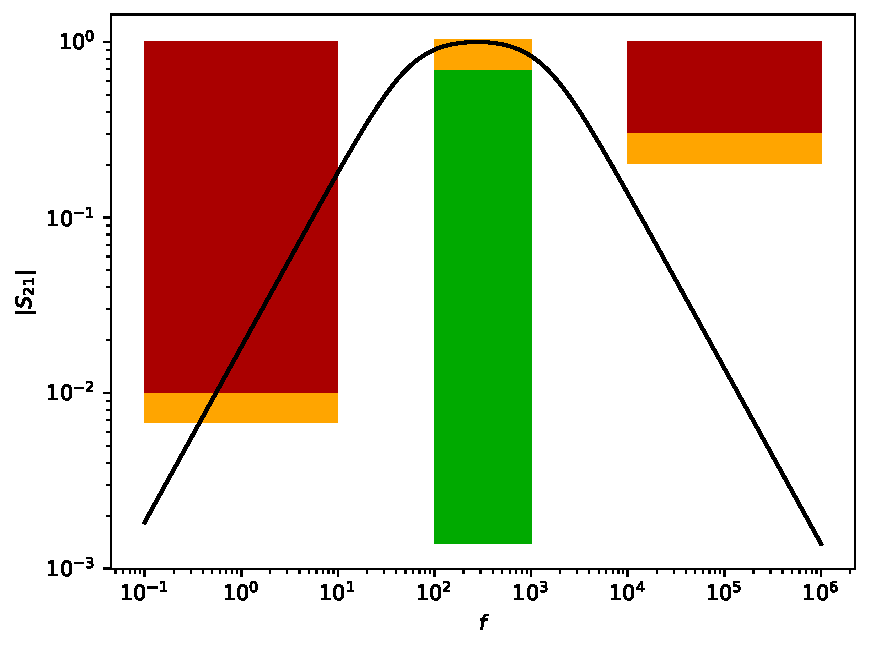
\includegraphics[width=0.7\textwidth]{atvitel_pelda.pdf}
            \caption{Három specifikált frekvenciasáv, két záró (piros) és egy áteresztő (zöld) sáv, valamint a büntetett margó használata.}
            \label{fig:margin}
        \end{figure}
        Az ábrán a bal oldali (kisebb frekvenciákhoz tartozó) záró sávban jól láthatóan az eredeti specifikáció által definiált tiltott régióba is belelóg az átviteli függvény. Emiatt természetesen ennek a sávnak nemnulla hozzájárulása van a célfüggvényhez. Az áteresztő sávban az eredeti specifikációnak ugyan megfelel az átviteli függvény, de a margóba még belóg, így itt is nemnulla büntetés adódik. A jobb oldali záró sávnak még a margóját is elkerüli az átviteli függvény, így ennek a sávnak 0 a célfüggvényhez a hozzájárulása.

        A margó bevezetését az indokolta, hogy jobban fel lehessen oldani az olyan helyzeteket, amikor az átviteli függvény ugyan teljesíti az eredeti specifikációt, de egyes frekvenciákon csak éppen, mivel ilyenkor valós alkalmazásoknál érdemes valamennyi tartalékot rászámolni a tervezésnél. Ilyenkor a margó lehetővé teszi, hogy nagyjából egyforma mértékben közelítse meg a határértékeket az átviteli függvény, ne pedig az egyiknél nagyon nagy tartalékkal, a másiknál pedig kis tartalékkal haladjon el. A margó célszerű használatakor olyan megoldás születik, amikor a megfelel a hálózat a specifikációnak, de a legtöbb sávhoz tartozó margóba kicsivel belelóg. Erre mutat példát \aref{fig:megoldas}. ábra, még ha csak egy nagyon egyszerű esetre is, amit az optimalizáló algoritmus talált meg.
        \begin{figure}[h!]
            \centering
            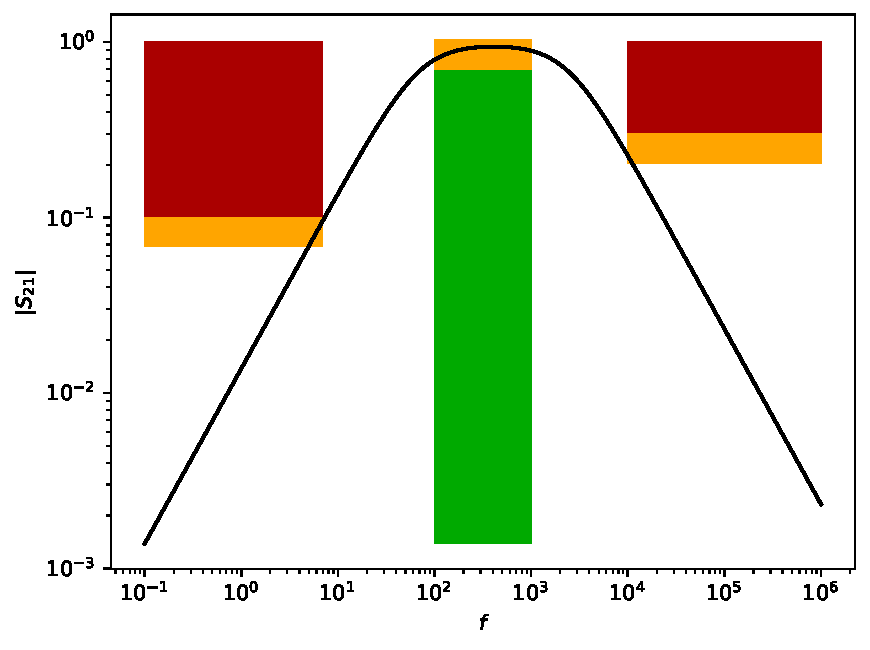
\includegraphics[width=0.7\textwidth]{megoldas.pdf}
            \caption{A margó ideális használata.}
            \label{fig:megoldas}
        \end{figure}

\section{Példák}

Az előző fejezetben egy sáváteresztő jellegű szűrőn keresztül mutattuk be a margókat, ebben a részben néhány további szűrőtípus optimalizálását mutatjuk be. Az egyik eset egy egyszerűbb aluláteresztő szűrő, a másik egy összetettebb, záró-áteresztő-záró-áteresztő struktúra.

	\subsection{Aluláteresztő szűrő}
		Egy ilyen szűrőtípus esetén egy áteresztő és egy zárósávot kell definiálnunk, közte egy toleranciasávval -- ennek hiányában nem adható helyes megoldás. Egy ilyen egyfokozatú szűrőnél legegyszerűbb esetben egyetlen elemet kell felhasználnunk, ez azonban nem biztosít elég meredek szűrőkarakterisztikát, továbbá túlzottan lekorlátozza a megoldható problémák halmazát.
		
		Ha kételemű aluláteresztő szűrőt tervezünk, egy párhuzamos kondenzátor és egy soros tekercset kell méreteznünk. Ennek a szemléletes magyarázata, hogy kis frekvenciákon a kondenzátornak nagy, a tekercsnek kicsi impedanciája van, ezáltal kis csillapítást okoz, nagy frekvenciákra pedig fordítva, jelentős csillapítást okoz. A specifikált frekvenciatartományokat, a megválasztott limiteket és a frekvenciatartományok típusát az alábbi kódrészlet mutatja.
		\begin{lstlisting}
starts = [0.1, 400e3]
ends = [100e3, 10e6]
limits = [0.2, 0.4]
directions = ["pass", "stop"]
spec = Spec(starts, ends, limits, directions, margin=0.47, n=1000)
		\end{lstlisting}
		Felveszünk $L = \SI{1}{mH}$ és $C = \SI{1}{\mu F}$ paraméter értékeket kiindulásnak, de az eredmény \ref{fig:alulatereszto}. ábrán láthatóan nem felel meg a követelményeknek.
		\begin{figure}[h!]
            \centering
            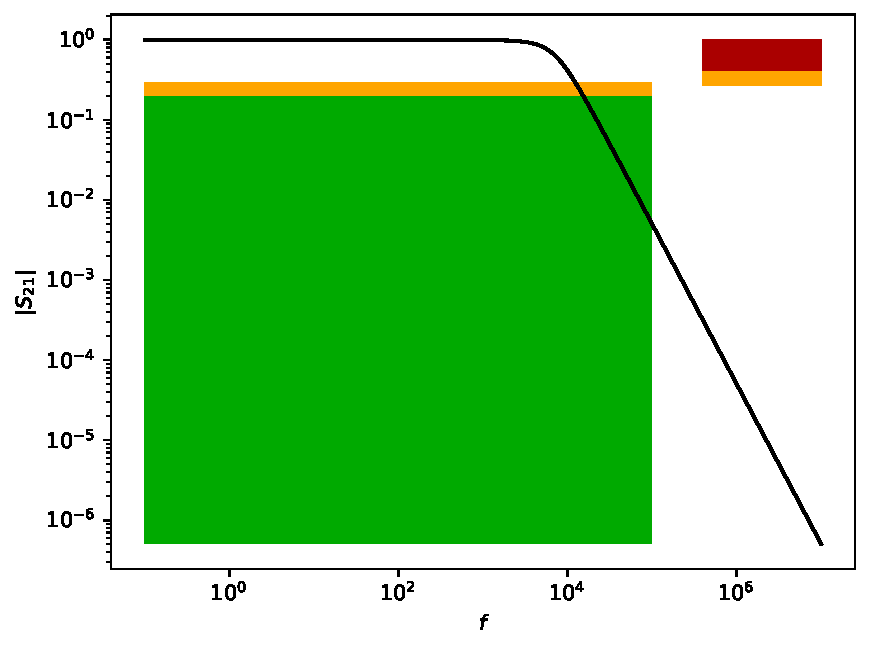
\includegraphics[width=0.7\textwidth]{alulatereszto.pdf}
            \caption{Aluláteresztő szűrő kezdeti paraméterekkel.}
            \label{fig:alulatereszto}
        \end{figure}
        Meghívjuk ezután az optimalizálót, úgy, hogy a paramétereket az inicializált értékének $\pm 1$ dekádos tartományában keresse, a határok megadását mutatja az alábbi kódrészlet.
        \begin{lstlisting}
bounds = {'par1C': (math.log(1e-7), math.log(1e-4)), 'ser1L': (math.log(1e-4), math.log(1e-2))}
        \end{lstlisting}
        Az eredményül adódott szűrőkarakterisztikát a \ref{fig:alulatereszto_opt}. ábra mutatja -- megjegyezzük, hogy ennek a méretezését kézzel is meg lehet tenni. Az $L$ és $C$ paraméterek egyikének lefixálása után a Thomson-formulát kell használni: $f_{rez} = \frac{1}{2\pi\sqrt{L C}}$, ami megadja a rezonanciafrekvenciát, esetünkben a töréspontot.
        \begin{figure}[h!]
            \centering
            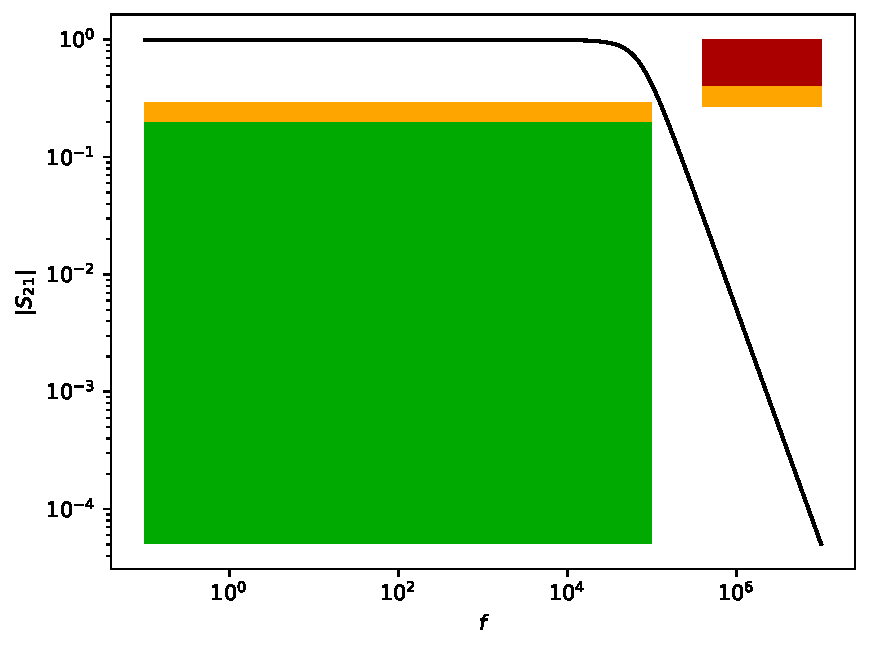
\includegraphics[width=0.7\textwidth]{alulatereszto_opt.pdf}
            \caption{Aluláteresztő szűrő optimalizált paraméterekkel, ami így megfelel a specifikációnak.}
            \label{fig:alulatereszto_opt}
        \end{figure}
        
	\subsection{Összetett példa}
		Vizsgáljunk meg egy összetettebb példát, ahol záró-áteresztő-záró-áteresztő sávok vannak, meglehetősen keskeny toleranciasávval elválasztva. A frekvenciatartományok kezdeteit, végeit, a limiteket és a sávok típusait a következőképp választottuk meg:
		\begin{lstlisting}
starts = [1, 2e4, 20e6, 200e6]
ends = [7e3, 12e6, 100e6, 1e9]
limits = [0.1, 0.7, 0.05, 0.1]
directions = ["stop", "pass", "stop", "pass"]
spec = Spec(starts, ends, limits, directions, margin=0.47, n=1000)
        \end{lstlisting}		
		Az első zárósáv $\SI{7}{kHz}$-es vége és következő áteresztő sáv $\SI{2}{MHz}$-es kezdete között egy felülátersztő jellegű, az előzőhöz hasonló kételemű blokkot használunk. A különbség itt a felüláteresztő viselkedés, azaz kis frekvenciákra kis átvitelt követelünk meg, ezt egy párhuzamos tekercsel és egy soros kondenzátorral tehetjük meg. A második fokozatban egy sávzáró szűrőt valósítunk meg, ugyanis a harmadik tartományunk előtt és után is áteresztőtartományok vannak. Ehhez első körben egy soros $LC$ kört használunk, azaz a párhuzamos ág elemeire nincs szükség. Egy soros $LC$ kör rezonanciafrekvencián nagy impedanciát mutat -- ideális esetben végtelen nagyot -- ami kis átvitelt, tehát az $|S_{21}|$ grafikonon egy leszívást mutat.

        A fent látható inicializálóértékekkel a szűrőkarakterisztika elmetszi a záró és az áteresztő sávokat, amint azt a \ref{fig:bonyi}. ábrán láthatjuk. Válasszuk meg a határokat, majd engedjük rá az optimalizálót.
        \begin{figure}[h!]
            \centering
            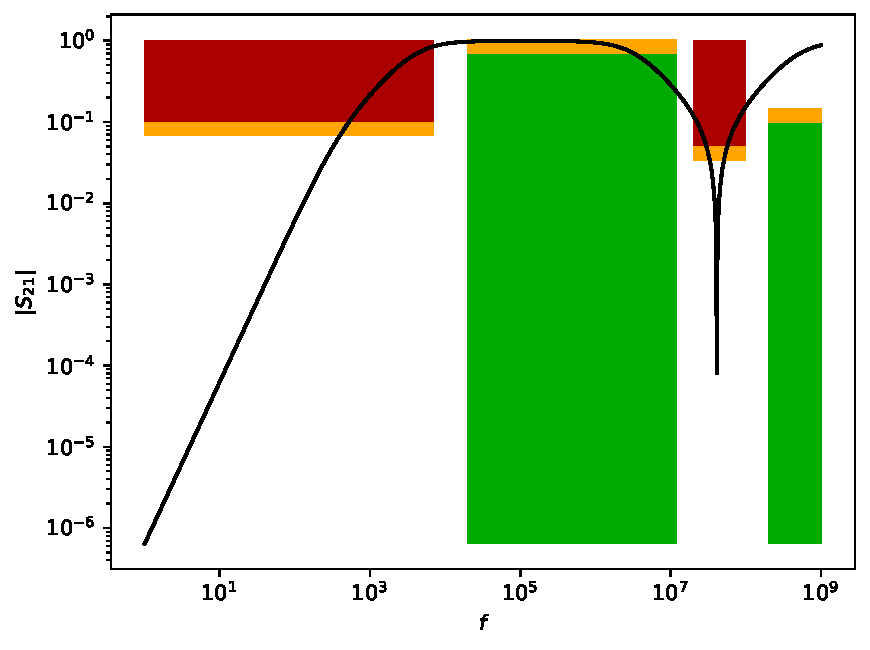
\includegraphics[width=0.7\textwidth]{bonyi.pdf}
            \caption{Összetett szűrő kezdeti paraméterekkel.}
            \label{fig:bonyi}
        \end{figure}
       	\begin{lstlisting}
spec.cost(plot=True, par1L = math.log(9e-4), ser1C = math.log(9e-6), ser2L = math.log(5e-6), ser2C = math.log(3e-12))
        \end{lstlisting}
        A \ref{fig:bonyi_subopt}. ábrán látható eredmény optimális, de nem helyes, a szűrőkarakterisztika mindkét zárótartományt elmetszi. A középső áteresztősávot viszont helyesen kikerüli, továbbá az első zárósávba is minimalizálta a belógást. Ezt akár meg is lehet szüntetni, ha meredekebb, 3 elemű felüláteresztő szűrő méretezünk rá, a sávzárónál ez már nem ilyen könnyű. Vélhetően specifikáció követel meg túl sokat, a további leszívások, azaz soros $LC$ tagból álló fokozatok beiktatása javulást még okozhat, de a maradéktalan betartás nehéz lenne.
        \begin{figure}[h!]
            \centering
            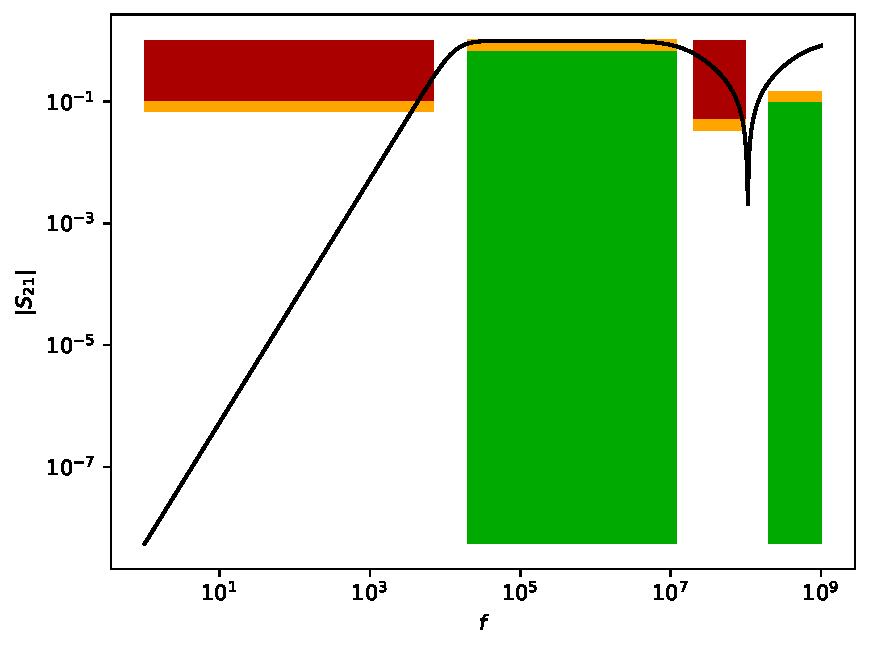
\includegraphics[width=0.7\textwidth]{bonyi_subopt.pdf}
            \caption{Összetett szűrő optimalizálás után. Látható, hogy az általunk megadott lehetőségekkel nem lehet megfelelni a követelményeknek.}
            \label{fig:bonyi_subopt}
        \end{figure}
        
        
        A második példa arra világít rá, hogy a neurális hálós optimalizáló nem csodaszer, csak a kezelője által meghatározott tartományon tud optimalizálni a megadott komplexitásig. A méretezés hosszadalmas folyamatát le tudja rövidíteni, de a tervező dolga figyelembe venni a szűrőkarakterisztika alapvető tulajdonságait.

\clearpage
\begin{thebibliography}{9}
    \bibitem{lancpar_spar} Láncparaméter -- S-paraméter konverzió (elérve 2023.06.07.): \url{https://www.rfwireless-world.com/Terminology/abcd-matrix-vs-s-matrix.html}
    \bibitem{bayesian_optimization} BayesianOptimization python könyvtár GitHub oldala. (Elérve: 2023.06.07.) \url{https://github.com/bayesian-optimization/BayesianOptimization}
    \bibitem{scipy} Scipy: L-BFGS-B minimalizáció dokumentációja \url{https://docs.scipy.org/doc/scipy/reference/optimize.minimize-lbfgsb.html}
	\bibitem{Z_to_ABCD} Párhuzamos admittancia és soros impedancia átszámolása láncparaméterekké. (Elérve: 2023.06.09.) \url{https://catalogimages.wiley.com/images/db/pdf/9780470183106.excerpt.pdf}
\end{thebibliography}

\clearpage
\appendix
\section{Az általunk írt specifikáció osztály}
	\lstinputlisting{../software/LC_opt_defs.py}
\end{document}
%%%% refs
% abcd to s parameters: https://www.rfwireless-world.com/Terminology/abcd-matrix-vs-s-matrix.html
